\documentclass{article}
\usepackage{amsmath}
\usepackage[mathletters]{ucs}
\usepackage[utf8x]{inputenc}
\usepackage[margin=1.5in]{geometry}
\usepackage{enumerate}
\newtheorem{theorem}{Theorem}
\usepackage[dvipsnames]{xcolor}
\usepackage{pgfplots}
\pgfplotsset{compat=1.18}
\setlength{\parindent}{0cm}
\usepackage{graphics}
\usepackage{graphicx} % Required for including images
\usepackage{subcaption}
\usepackage{bigintcalc}
\usepackage{pythonhighlight} %for pythonkode \begin{python}   \end{python}
\usepackage{appendix}
\usepackage{arydshln}
\usepackage{physics}
\usepackage{booktabs} 
\usepackage{adjustbox}
\usepackage{mdframed}
\usepackage{relsize}
\usepackage{physics}
\usepackage[thinc]{esdiff}
\usepackage{esint}  %for lukket-linje-integral
\usepackage{xfrac} %for sfrac
\usepackage{hyperref} %for linker, må ha med hypersetup
\usepackage[noabbrev, nameinlink]{cleveref} % to be loaded after hyperref
\usepackage{amssymb} %\mathbb{R} for reelle tall, \mathcal{B} for "matte"-font
\usepackage{listings} %for kode/lstlisting
\usepackage{verbatim}
\usepackage{graphicx,wrapfig,lipsum,caption} %for wrapping av bilder
\usepackage{mathtools} %for \abs{x}
\usepackage[norsk]{babel}
\usepackage{cancel}
\definecolor{codegreen}{rgb}{0,0.6,0}
\definecolor{codegray}{rgb}{0.5,0.5,0.5}
\definecolor{codepurple}{rgb}{0.58,0,0.82}
\definecolor{backcolour}{rgb}{0.95,0.95,0.92}
\lstdefinestyle{mystyle}{
    backgroundcolor=\color{backcolour},   
    commentstyle=\color{codegreen},
    keywordstyle=\color{magenta},
    numberstyle=\tiny\color{codegray},
    stringstyle=\color{codepurple},
    basicstyle=\ttfamily\footnotesize,
    breakatwhitespace=false,         
    breaklines=true,                 
    captionpos=b,                    
    keepspaces=true,                 
    numbers=left,                    
    numbersep=5pt,                  
    showspaces=false,                
    showstringspaces=false,
    showtabs=false,                  
    tabsize=2
}

\lstset{style=mystyle}
\author{Oskar Idland}
\title{Oblig 3}
\date{}
\begin{document}
\maketitle
\newpage

\section*{Problem 3.1 (L)}


\section*{Problem 3.2 (L)}
As a continuous observable have an infinite amount of possible measurement values, yet can't be in two states at once, we need an infinite-dimensional Hilbert space. All the state vectors need to be linearly independent, and an infinite amount of linearly independent vectors must be in a infinite-dimensional Hilbert space.

\section*{Problem 3.3 (L)}
The probability of measuring the the value $g$:
\[
P(g) = \left|\bra{g}\ket{ψ}\right|^2 = \frac{1}{2}\left(-ia +   ib\right)^2 = \frac{1}{2} \left(a^2 - b^2\right)  
\]

If we measure the observable to be $g$, there is a 100\% of the state being $\ket{g}$. If $g$ was not obtained then there is a 0\% chance of the state being $\ket{g}$.  


\section*{Problem 3.4 (L)}
As this is a degenerate state of value 2, there are two possible eigenstates which can result in measuring +1. The probability of measuring +1 is the sum of the probabilities of measuring +1 for each of the eigenstates. 
\[
\hat{P}_1 = \left|a_1\right|^2 + \left|a_2\right|^2 
\]

\section*{Problem 3.5 (L)}
\colorbox{red}{TODO:}

\section*{Problem 3.6 (H)}
\subsection*{a)}
It is easy to see that $\hat{H} = \hat{H}^{†}$. Now we have to check if it has real eigenvalues. 
\[
\hat{H} = 
\begin{pmatrix}
 1 & \frac{i}{2} & 0 \\
 -\frac{i}{2} & 1 & 0 \\
 0 & 0 & \frac{1}{2} \\
\end{pmatrix}
\]
Now we employ the eigenvalue equation:
\[
\det \left(\hat{H} - \lambda \hat{I}\right) = 0
\]
\[
\det \left(
\begin{pmatrix*}[r]
 1-λ & \frac{i}{2} &0 \\
 -\frac{i}{2} & 1 - λ & 0 \\
 0 & 0 & \frac{1}{2} - λ \\
\end{pmatrix*}
\right)
\]
\[
\underbrace{(1-λ) (1 - λ)\left(\frac{1}{2} - λ\right)}_{\text{term 1}} -\underbrace{ \frac{i}{2} \left( - \frac{i}{2} \left(\frac{1}{2} - λ\right)\right)}_{\text{term 2}} + 0 = 0
\]
Beginning with the first term:
\[
(1 - 2λ + λ^2)\left(\frac{1}{2} - λ\right) = \frac{1}{2} - λ + \frac{λ^2}{2} - λ + 2λ^2 - λ^3 
\]
\[
\underline{\frac{1}{2} - 2λ + \frac{5}{2}λ^2 - λ^3}
\]
Now the second term:
\[
- \frac{1}{4} \left(\frac{1}{2} - λ\right) = \underline{- \frac{1}{8} + \frac{λ}{4}}
\]
\[
\frac{1}{2} - 2λ + \frac{5}{2}λ^2 - λ^3 - \frac{1}{8} + \frac{λ}{4} = 0
\]
\[
-λ^3 + \frac{5}{2}λ^2 - \frac{7}{4}λ - \frac{3}{8} = 0
\]
\[
\underline{\underline{λ = \frac{3}{2} \quad , \quad λ   = \frac{1}{2} \quad , \quad λ = -\frac{1}{2}}}
\]
All the eigenvalues are real, and the matrix is hermitian.

\subsection*{b)}
\[
\hat{H}\ket{1} = \frac{1}{\sqrt{2}} 
\begin{pmatrix*}[r]
    1 & \frac{i}{2} & 0 \\
    -\frac{i}{2} & 1 & 0 \\
    0 & 0 & \frac{1}{2} \\
\end{pmatrix*}
\begin{pmatrix*}[r]
 i \\
 1 \\
 0 \\
\end{pmatrix*} 
\]
\[
\frac{1}{\sqrt{2}}
\begin{pmatrix*}[r]
 i + \frac{i}{2} + 0 \\
 -\frac{i}{2}i + 1 + 0 \\
 0 + 0 + 0 \\
\end{pmatrix*}
\]
\[
\frac{1}{\sqrt{2}}
\begin{pmatrix*}[r]
\frac{3}{2}i \\
\frac{3}{2} \\
0 \\
\end{pmatrix*} = \frac{1}{\sqrt{2}} \frac{3}{2}
\begin{pmatrix*}[r]
i \\
1 \\
0 \\
\end{pmatrix*}
\]
$\ket{1}$ is an eigenvector with eigenvalue $\frac{3}{2}$.

\[
\hat{H}\ket{2} = 
\begin{pmatrix*}[r]
1 & \frac{i}{2} & 0 \\
-\frac{i}{2} & 1 & 0 \\
0 & 0 & \frac{1}{2} \\
\end{pmatrix*}
\begin{pmatrix*}[r]
0 \\
0 \\
1 \\
\end{pmatrix*}
\]
\[
\begin{pmatrix*}[r]
0 \\
0 \\
\frac{1}{2} \\
\end{pmatrix*} = \frac{1}{2} 
\begin{pmatrix*}[r]
0 \\
0 \\
1 \\
\end{pmatrix*}
\]
$\ket{2}$ is an eigenvector with eigenvalue $\frac{1}{2}$.

\[
\hat{H}\ket{3} = \frac{1}{\sqrt{3}}
\begin{pmatrix*}[r]
1 & \frac{i}{2} & 0 \\
-\frac{i}{2} & 1 & 0 \\
0 & 0 & \frac{1}{2} \\
\end{pmatrix*}
\begin{pmatrix*}[r]
-i \\
1 \\
-1 \\
\end{pmatrix*}
\]
\[
\frac{1}{\sqrt{3}}
\begin{pmatrix*}[r]
-i + \frac{i}{2} + 0 \\
- \frac{i}{2}i + 1 + 0 \\
0 + 0 - \frac{1}{2} \\
\end{pmatrix*} = \frac{1}{\sqrt{3}} \frac{1}{2}
\begin{pmatrix*}[r]
-i \\
1 \\
-1 \\
\end{pmatrix*}
\]
$\ket{3}$ is an eigenvector with eigenvalue $\frac{1}{2}$.

\subsection*{c)} 
The operator $\hat{H}$ can br written using the eigenstates as a basis $\hat{H}_{E}$
\[
H_{11} = \bra{1}\hat{H}\ket{1} = \frac{3}{2} \bra{1}\ket{1} = \frac{3}{2}
\]
As the matrix eigenstates must be orthogonal, we only need to calculate the diagonal elements, where $i = j$. 
\[
H_{22} = \bra{2}\hat{H}\ket{2} = \frac{1}{2} \bra{2}\ket{2} = \frac{1}{2}
\]
\[
H_{33} = \bra{3}\hat{H}\ket{3} = \frac{1}{2} \bra{3}\ket{3} = \frac{1}{2}
\]
\[
\hat{H}_{E} = 
\begin{pmatrix*}[r]
\frac{3}{2} & 0 & 0 \\
0 & \frac{1}{2} & 0 \\
0 & 0 & \frac{1}{2} \\
\end{pmatrix*}
\]
This is of course an diagonal matrix, and the eigenvalues are the diagonal elements.

\subsection*{d)}
\colorbox{red}{TODO: Are they not already orthogonal?}

\newpage
\section*{Problem 3.7 (H)}
\subsection*{a)}
\[
\hat{H} = -g ∑_{i=0}^{L-2} \left(\ket{i}\bra{i+1} + \bra{i+1}\ket{i}\right)-  V \ket{0}\bra{0}
\]
\[
\hat{H} = -g \left(\ket{0}\bra{1} + \ket{1}\bra{0} + \ket{1}\bra{2} + \ket{2}\bra{1} + \ket{2}\bra{3} + \ket{3}\bra{2} \right) - V \ket{0}\bra{0}   
\]
Lets expand one term at a time. 
\[
\ket{0}\bra{1} = 
\begin{pmatrix*}[r]
 0 & 1 & 0 & 0 \\
 0 & 0 & 0 & 0 \\
 0 & 0 & 0 & 0 \\
 0 & 0 & 0 & 0 \\
\end{pmatrix*} \quad , \quad \ket{1}\bra{0} = 
\begin{pmatrix*}[r]
 0 & 0 & 0 & 0 \\
 1 & 0 & 0 & 0 \\
 0 & 0 & 0 & 0 \\
 0 & 0 & 0 & 0 \\
\end{pmatrix*}
\]
\[
\ket{1}\bra{2} = 
\begin{pmatrix*}[r]
 0 & 0 & 0 & 0 \\
 0 & 0 & 1 & 0 \\
 0 & 0 & 0 & 0 \\
 0 & 0 & 0 & 0 \\
\end{pmatrix*} \quad , \quad \ket{2}\bra{1} =
\begin{pmatrix*}[r]
 0 & 0 & 0 & 0 \\
 0 & 0 & 0 & 0 \\
 0 & 1 & 0 & 0 \\
 0 & 0 & 0 & 0 \\
\end{pmatrix*}
\]
\[
\ket{2}\bra{3} =
\begin{pmatrix*}[r]
 0 & 0 & 0 & 0 \\
 0 & 0 & 0 & 0 \\
 0 & 0 & 0 & 1 \\
 0 & 0 & 0 & 0 \\
\end{pmatrix*} \quad , \quad \ket{3}\bra{2} =
\begin{pmatrix*}[r]
 0 & 0 & 0 & 0 \\
 0 & 0 & 0 & 0 \\
 0 & 0 & 0 & 0 \\
 0 & 0 & 1 & 0 \\
\end{pmatrix*}
\]
\[
\ket{0}\bra{0} = 
\begin{pmatrix*}[r]
 1 & 0 & 0 & 0 \\
 0 & 0 & 0 & 0 \\
 0 & 0 & 0 & 0 \\
 0 & 0 & 0 & 0 \\
\end{pmatrix*}
\]
\[
\hat{H} =
\begin{pmatrix*}[r]
 -V & -g & 0 & 0 \\
 -g & 0 & -g & 0 \\
 0 & -g & 0 & -g \\
 0 & 0 & -g & 0 \\
\end{pmatrix*}
\]

\subsection*{b)}
The position operator $\hat{X}$ in matrix form:
\[
\hat{X} = 
\begin{pmatrix*}[r]
 0 & 0 & 0 & 0 \\
 0 & 1 & 0 & 0 \\
 0 & 0 & 2 & 0 \\
 0 & 0 & 0 & 3 \\
\end{pmatrix*}
\]

\subsection*{c)}

\begin{figure}[h!]
\centering
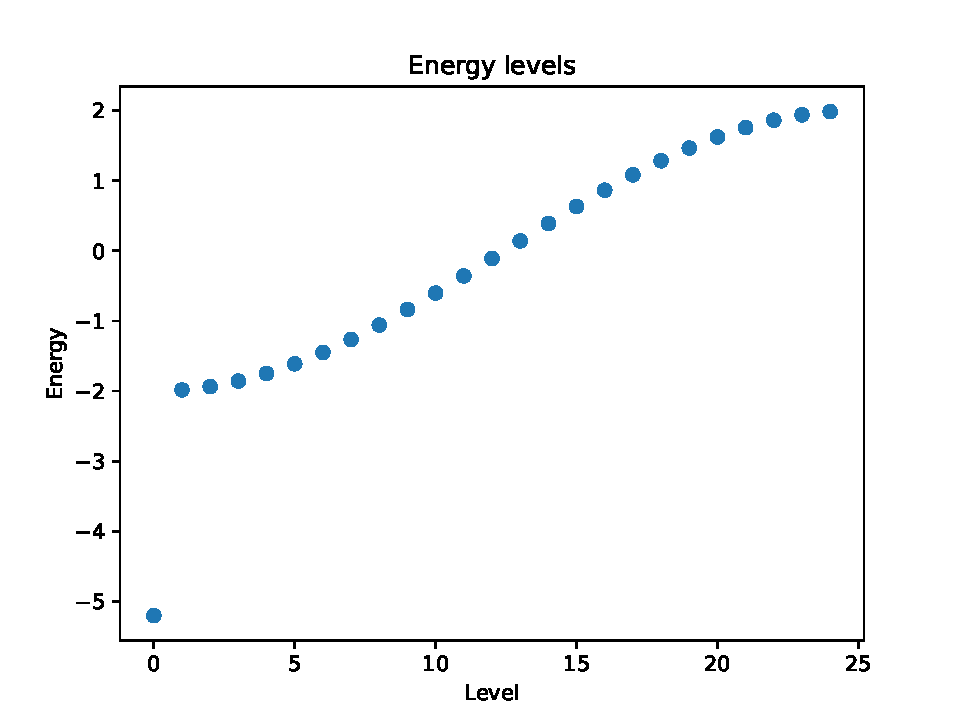
\includegraphics[width = .75\textwidth]{energy_levels.pdf}
\caption{Plot of the energy levels}
\label{fig: energy_levels}
\end{figure}
The lowest energy level was approximately $E_0 = -5.2$. 

\subsection*{d)}
The energy eigenkets contains the information about the probability of finding the particle in a given state. Each eigenket correspond to each position, and each index correspond to each energy level. The probability of finding the particle in position 0 in the ground state, is the absolute value squared of the first element, in the first eigenket. The probability of finding the particle in position 1 in the ground state, is the absolute value squared of the first element, in the second eigenket. This turns out to be 96\% and 39\% respectively. 


\subsection*{e)}
We set our state vector $\ket{Ψ}$ to be in position 0. The we evolve it over time with the time evolution operator $\hat{U}$, defined as: 
\[
\hat{U} = e^{-i\hat{H}t / ℏ}
\]
This gives us and expression for the stationary state $\ket{ψ_0}$ as follows:
\[
\ket{ψ_0} = ∑_{n}^{L} c_n(t)\ket{E_n} 
\]
Where $c_n$ is the coordinates of the state vector in the energy eigenbasis and $\ket{E_n}$ is the energy eigenkets. We calculate the coordinates $c_n$ like this:
\[
c_n = \bra{E_n}\ket{Ψ}
\]
Now we can calculate the time evolution of the state vector: 
\[
\ket{Ψ(t)} = ∑_{n}^{L} \left|c_n(t)\right|^2 U \ket{E_n} 
\]
We can the plot the probability of finding the particle at position 0 as a function of time, by taking the absolute value squared of the state vector. 
 
As we already know it is at position 0, we can use $\begin{pmatrix} 1_1 \\ 0_2 \\ \vdots \\ 0_L \end{pmatrix}$ instead of $\ket{Ψ(0)}$.

\begin{figure}[h!]
\centering
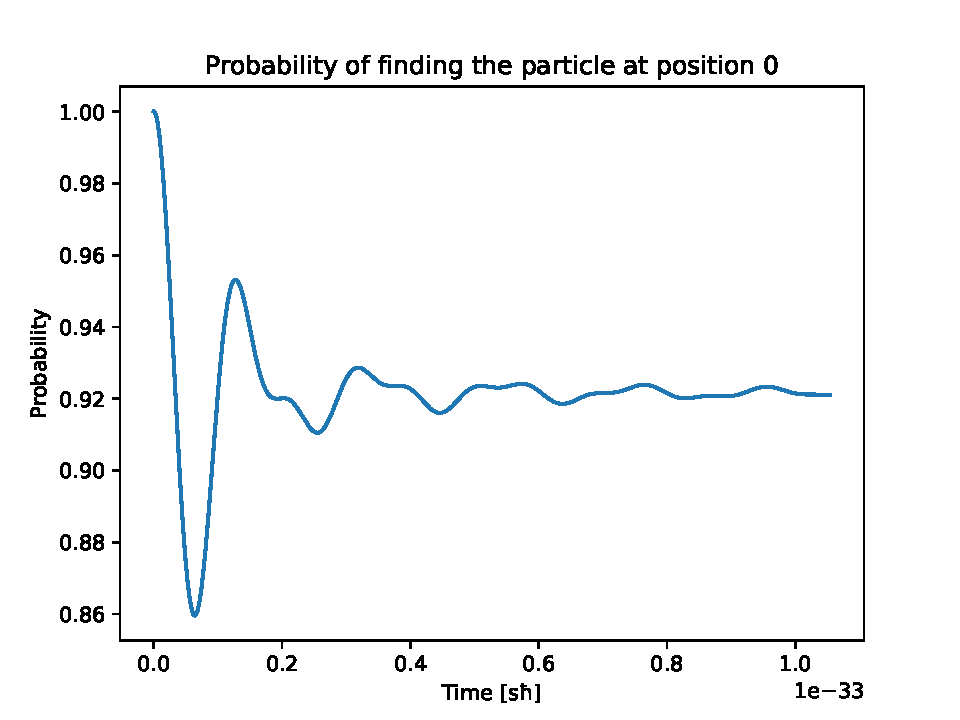
\includegraphics[width = .75\textwidth]{probability.pdf}
\caption{Probability of finding the particle at position 0 as a function of time}
\label{fig: probability}
\end{figure}


\section*{3.8 (X)}
\colorbox{red}{TODO:}
\subsection*{a)}

\subsection*{b)}



\end{document}